\documentclass[12pt,compress]{beamer}
\usepackage{amsmath}
\usepackage{cmbright}
\usepackage{url}
\usepackage{ucs}
\usepackage[utf8x]{inputenc}
\usepackage[ngerman]{babel}
\usepackage{bbm}
\usepackage{ulem}
\usepackage{multicol}
\usepackage{comment}
\usepackage{setspace}
\usepackage{color}
\usepackage{movie15}
\usepackage{hyperref}
\usepackage{bookman}

\usetheme{Boadilla}
\setbeamertemplate{footline}%{infolines theme}

\usecolortheme{lily}
\usefonttheme{serif}
\useinnertheme{circles}
\setbeamercovered{transparent}
\beamertemplatenavigationsymbolsempty

\definecolor{darkgreen}{rgb}{0,0.5,0}

\hypersetup{
    bookmarks=true,
    unicode=true,
    pdftoolbar=true,
    pdfmenubar=true,
    pdffitwindow=false,
    pdfstartview={FitH},
    pdftitle={Klassisches Chaos und Poincaré-Schnitte},
    pdfauthor={Michael Hartmann},
    pdfsubject={Vortrag über klassisches Chaos in hamiltonschen Systemen am Beispiel des Doppelpendels},
    pdfcreator={vim},
    pdfproducer={pdflatex},
    pdfkeywords={Doppelpendel} {Chaos} {Poincare},
    pdfnewwindow=true,
    colorlinks=true,
    linkcolor=black,
    citecolor=green,
    filecolor=magenta,
    urlcolor=darkgreen
}



\title{Was ist Chaos? }
%\subtitle{Einführung am Beispiel des Doppelpendels}
\institute{Theoretische Physik I}
\author{Michael Hartmann}
\date{18. November 2015}


\titlegraphic{\includegraphics[scale=0.4]{images/title.png}}


\begin{document}

\begin{frame}
    \titlepage
\end{frame}


\section{Was ist ein Doppelpendel?}


\frame {
    \frametitle{Was ist ein Doppelpendel?}

    \begin{minipage}[b]{0.4\textwidth} 
    \includegraphics[scale=1]{images/sketch.pdf}
    
    \end{minipage}
    \hfill
    \begin{minipage}[b]{0.4\textwidth}
    \begin{align}
    \nonumber
    x_1 &= l \sin\theta_1 \\
    \nonumber
    y_1 &= -l \cos\theta_1 \\
    \nonumber
    x_2 &= l \sin\theta_1 + l \sin\theta_2 \\
    \nonumber
    y_2 &= -l \cos\theta_1 - l \cos\theta_2
    \end{align}
    \end{minipage}
}

\frame {
    \frametitle{Was ist ein Doppelpendel?}

    \begin{center}
    \includemovie[poster,autoplay,controls=true]{7.5cm}{7.5cm}{videos/pendulum.mp4}
    \end{center}
}

\section{Bewegungsgleichungen}

\section{Poincaré-Schnitte}

\frame {
    \frametitle{Poincaré-Schnitte}

    \begin{center}
    \includegraphics[scale=0.45]{images/poincare_idea.png}
    \includegraphics[scale=0.45]{images/poincare_cycle3.png}
    \end{center}

    \hfill
    \hrule
    \ \\
    {\footnotesize Bildquelle: An Exploration of Chaos, Argyris, Faus, Haase}
}

\frame {
    \frametitle{Vorteile von Poincaré-Schnitten}

    \begin{itemize}
        \item Vergleich verschiedener Anfangsbedingungen
        \item Reduktion der Dimension ohne Verlust an Informationen
        \item qualitatives Verhalten:
        \begin{itemize}
            \item Fixpunkte entsprechen periodische Orbits
            \item Unterscheidung chaotischer und regulärer Bereiche
            \item Linien entsprechen quasiperiodischer Orbits
        \end{itemize}
    \end{itemize}
}

\frame {
    \frametitle{Poincaré-Schnitte für das Doppelpendel}

    \begin{itemize}
        \item abhängig von Parametern: $E$, $L_1$, $L_2$
        \item 4 Freiheitsgrade: 2 Impulse, 2 Winkel
        \item Energieerhaltung: Trajektorien auf Hyperfläche eingeschränkt
        \item Poincaré-Bedingung $\theta_2 = 0$: noch zwei Variablen
        \item Abbildung von Punkten: $$P(\theta_1^{(0)}, p_1^{(0)}) \mapsto (\theta_1^{(1)}, p_1^{(1)})$$
        \item Durchstoßrichtung beachten!
    \end{itemize}

}

\frame {
    \frametitle{Poincaré-Schnitt für $E=15$}

    \begin{center}
    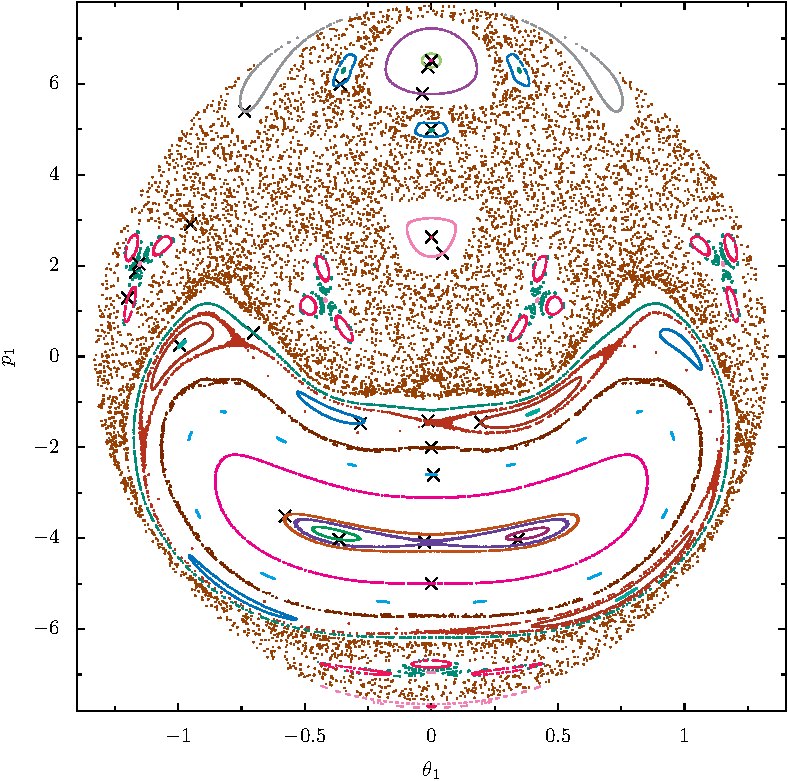
\includegraphics[width=0.65\textwidth]{plots/E=15.pdf}
    \end{center}
}

\frame {
    \frametitle{Fixpunkte im Poincaré-Schnitt}

    \begin{minipage}[b]{0.3\textwidth} 
    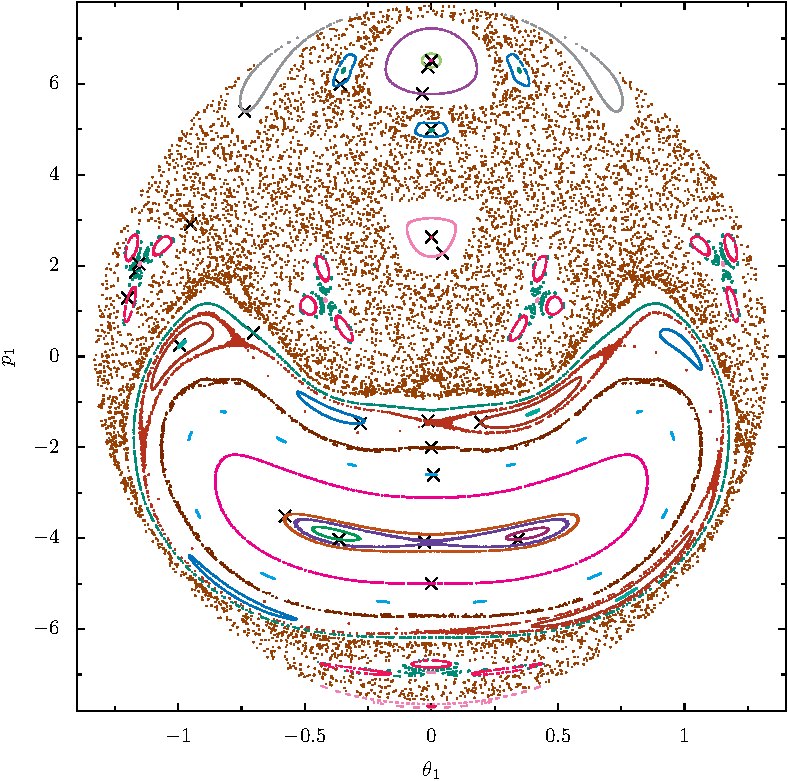
\includegraphics[scale=0.35]{plots/E=15.pdf}
    \end{minipage}
    \hfill
    \begin{minipage}[b]{0.6\textwidth}
    \begin{itemize}
    \item Elliptische Fixpunkte
    \begin{itemize}
    \item Orbit stabil
    \end{itemize}
    \item Hyperbolische Fixpunkte
    \begin{itemize}
    \item Orbit instabil
    \item liegt im chaotischen Bereich
    \item anfällig gegen Störungen
    \end{itemize}
    \item Chaos
    \end{itemize}
    \end{minipage}
}

\section{Beispiele}

\frame {
    \frametitle{Beispiel -- stabiler periodischer Orbit}

    \begin{center}
    \includemovie[poster,autoplay,controls=true]{7.5cm}{7.5cm}{videos/periodisch.mpeg}

    $E=15$, $\theta_1=0$, $p_1=2.63362868$
    \end{center}
}

\frame {
    \frametitle{Beispiel -- stabiler periodischer Orbit}

    \begin{center}
    \includemovie[poster,autoplay,controls=true]{7.5cm}{7.5cm}{videos/periodisch_kompliziert.mpeg}

    $E=15$, $\theta_1=0$, $p_1=-2.78854801$
    \end{center}
}

\frame {
    \frametitle{Beispiel -- instabiler periodischer Orbit}

    \begin{center}
    \includemovie[poster,autoplay,controls=true]{7.5cm}{7.5cm}{videos/periodisch_instabil.mpeg}

    $E=15$, $\theta_1=0$, $p_1=-4.10536235$
    \end{center}
}

\frame {
    \frametitle{Beispiel -- quasiperiodischer Orbit}

    \begin{center}
    \includemovie[poster,autoplay,controls=true]{7.5cm}{7.5cm}{videos/quasiperiodisch.mpeg}

    $E=15$, $\theta_1=0$, $p_1=-5$
    \end{center}
}

\frame {
    \frametitle{Beispiel -- Chaos}

    \begin{center}
    \includemovie[poster,autoplay,controls=true]{11cm}{5.5cm}{videos/chaos.mpeg}
    links: $E=15$, $\theta_1=0.8$, $p_1=-4$ \\
    rechts: $E=15$, $\theta_1=0.8$, $p_1=-4.01$
    \end{center}
}


\end{document}
